\documentclass[11pt]{article}
\usepackage[spanish,es-nodecimaldot,es-tabla]{babel}
% Preambulo comun de los tres documentos (el idioma de babel se carga antes de este archivo)
\usepackage[utf8]{inputenc}
\usepackage[T1]{fontenc}
\usepackage{lmodern}
\usepackage[margin=2.5cm]{geometry}
\usepackage{amsmath,amssymb}
\usepackage{graphicx}
\usepackage{array}
\usepackage{float}
\usepackage{caption}
\usepackage{enumitem}
\usepackage{microtype}
\usepackage[round]{natbib}
\usepackage[hidelinks]{hyperref}
\captionsetup{font=small,labelfont=bf,justification=justified,singlelinecheck=false}
\captionsetup[table]{position=top,skip=6pt}
\renewcommand{\arraystretch}{1.25}
\setlength{\parskip}{0.45em}
\setlength{\parindent}{0pt}
\graphicspath{{figuras/}}
\newcommand{\tabla}[1]{\centering\small\setlength{\tabcolsep}{4.5pt}\input{tablas/#1}}

% Titulos de tablas y figuras (espanol). Compartidos por los documentos y por las versiones PNG.
\newcommand{\capTabA}{Supervivencia de plántulas en LHS-1 según la proporción de sustrato ionitopónico. Los valores se expresan como media $\pm$ desviación estándar (DE); $n = 5$ unidades experimentales por grupo.}
\newcommand{\capTabB}{Análisis de varianza para la proporción de sustrato ionitopónico en LHS-1, particionado en dos contrastes ortogonales planificados.}
\newcommand{\capTabC}{Contrastes planificados para la supervivencia de plántulas en LHS-1. Las diferencias se expresan en puntos porcentuales (pp).}
\newcommand{\capTabD}{Sensibilidad de los contrastes planificados a la elección del término de error y de la unidad de análisis.}
\newcommand{\capTabE}{Contrastes de contexto para la supervivencia de plántulas. Las diferencias se expresan en puntos porcentuales (pp).}
\newcommand{\capTabF}{Análisis de varianza de dos vías para la supervivencia de plántulas según sustrato y tratamiento.}
\newcommand{\capTabG}{Germinación según tratamiento y sustrato. Los valores se expresan como proporciones con intervalos de confianza (IC) exactos (Clopper--Pearson) del 95\,\%.}
\newcommand{\capTabH}{Contrastes seleccionados para la germinación, evaluados a nivel de semilla y a nivel de unidad experimental.}
\newcommand{\capTabI}{Potencia estadística de la fase piloto y tamaño de muestra requerido para un experimento confirmatorio (potencia de 0.80, $\alpha = 0.05$).}
\newcommand{\capFigA}{Supervivencia de plántulas en LHS-1 según la proporción de sustrato ionitopónico. Los puntos representan las medias de grupo y las barras representan $\pm 1$ error estándar (error agrupado, 32 grados de libertad); $n = 5$ unidades experimentales por grupo.}
\newcommand{\capFigB}{Diferencias estimadas en la supervivencia de plántulas con intervalos de confianza bilaterales del 95\,\%. Los marcadores oscuros corresponden a los contrastes planificados de la hipótesis; los marcadores grises corresponden a comparaciones complementarias y de contexto.}
\newcommand{\capFigC}{Supervivencia de plántulas según tratamiento y sustrato. Los puntos representan las medias de grupo y las barras representan $\pm 1$ error estándar (error agrupado, 32 grados de libertad).}
\newcommand{\capFigD}{Germinación según tratamiento y sustrato. Los puntos representan las proporciones observadas y las barras representan intervalos de confianza exactos (Clopper--Pearson) del 95\,\%; 20 semillas por grupo.}
\newcommand{\capFigE}{Potencia estadística para detectar una diferencia de 20 puntos porcentuales en la supervivencia de plántulas en función del número de unidades experimentales por grupo ($\alpha = 0.05$; desviación estándar residual de 31.8 puntos porcentuales). La línea horizontal indica una potencia de 0.80.}
\newcommand{\capFigTA}{Distribución $t$ de Student con 32 grados de libertad bajo la hipótesis nula de C1. El estadístico observado no alcanza la región de rechazo unilateral.}
\newcommand{\capFigTB}{Distribución de permutación exacta de la diferencia de germinación entre el aditivo al 5\,\% y la solución convencional en LHS-1, con la unidad experimental como unidad de análisis (252 reordenamientos de 10 unidades). En azul, los reordenamientos al menos tan extremos como el observado.}


\title{\textbf{Análisis estadístico de la fase piloto}\\[4pt]
\large Supervivencia de plántulas y germinación de \textit{Raphanus sativus} en el simulante de regolito lunar LHS-1 enmendado con sustrato ionitopónico}
\author{}
\date{}

\begin{document}
\maketitle
\vspace{-3em}

\section{Análisis estadístico}

\subsection{Diseño experimental y datos}

Durante la fase piloto se evaluaron 160 semillas de \textit{Raphanus sativus} en 40 unidades experimentales, utilizando dos sustratos de crecimiento: el simulante de regolito lunar LHS-1 y arena de río autoclavada. Para cada sustrato se consideraron cuatro tratamientos nutricionales: control, solución nutritiva convencional, aditivo al 5\,\% y aditivo al 10\,\%. Este arreglo corresponde a un diseño factorial $2 \times 4$ con cinco unidades experimentales por combinación de sustrato y tratamiento, y cuatro semillas por unidad.

Los tratamientos con aditivo corresponden a la proporción de sustrato ionitopónico incorporada al medio de crecimiento (5\,\% y 10\,\%), mientras que el control corresponde al medio sin enmendar (0\,\%). La germinación se expresó como el porcentaje de semillas sembradas que germinaron en cada unidad, y la supervivencia como el porcentaje de semillas germinadas que sobrevivieron en cada unidad. El análisis se realizó a partir de los estadísticos resumen de cada combinación de sustrato y tratamiento (media $\pm$ desviación estándar de los porcentajes por unidad).

\subsection{Hipótesis y contrastes planificados}

Se planteó como hipótesis que las plantas cultivadas en el simulante enmendado mostrarían una mayor supervivencia que las cultivadas en LHS-1 sin enmendar, y que esta respuesta variaría con la proporción de sustrato ionitopónico en el medio de crecimiento. Sean $\mu_0$, $\mu_5$ y $\mu_{10}$ las medias de supervivencia en LHS-1 con 0\,\%, 5\,\% y 10\,\% de sustrato ionitopónico, respectivamente. La hipótesis se tradujo en dos contrastes ortogonales planificados:
\begin{align*}
\text{C1 (efecto de la enmienda):} \quad & H_0\colon \tfrac{1}{2}(\mu_5 + \mu_{10}) \le \mu_0 & \text{vs.} \quad & H_1\colon \tfrac{1}{2}(\mu_5 + \mu_{10}) > \mu_0,\\[2pt]
\text{C2 (dependencia de la proporción):} \quad & H_0\colon \mu_{10} = \mu_5 & \text{vs.} \quad & H_1\colon \mu_{10} \ne \mu_5.
\end{align*}
El componente de la hipótesis relacionado con el desarrollo de las plantas no se evaluó, dado que en el presente análisis no se incluyeron variables de desarrollo.

\subsection{Análisis de la supervivencia de plántulas}

La supervivencia de plántulas se analizó mediante un análisis de varianza (ANOVA) calculado a partir de las medias y desviaciones estándar de los grupos. La variación entre las tres proporciones de sustrato ionitopónico en LHS-1 (2 grados de libertad) se particionó en los contrastes C1 y C2 (1 grado de libertad cada uno). Como término de error se utilizó el cuadrado medio agrupado dentro de los grupos de las ocho combinaciones de sustrato y tratamiento (32 grados de libertad), dado que todas las unidades experimentales pertenecieron al mismo experimento y se manejaron bajo los mismos procedimientos.

Dado que C1 es direccional, se evaluó con una prueba $t$ unilateral; su valor $p$ bilateral se reporta también como referencia. C2 se evaluó con una prueba $t$ bilateral. Los valores $p$ de los dos contrastes planificados se ajustaron con el procedimiento de Holm \citep{holm}. Como análisis complementarios, cada proporción se comparó con el control sin enmendar, se estimó un conjunto de contrastes de contexto y se examinaron los efectos del sustrato, del tratamiento y de su interacción mediante un ANOVA de dos vías, seguido de la prueba de Tukey para las comparaciones entre tratamientos.

La robustez de los contrastes planificados se examinó de tres maneras: (i) estimando el error únicamente con los grupos involucrados en cada contraste; (ii) utilizando la aproximación de Welch--Satterthwaite, que no supone varianzas iguales \citep{welch,satterthwaite}; y (iii) repitiendo las comparaciones a nivel de semilla con pruebas exactas.

\subsection{Análisis de la germinación}

La germinación fue cercana al 100\,\% en la mayoría de los grupos y tres grupos no presentaron variabilidad; por lo tanto, un ANOVA sobre porcentajes no se consideró apropiado para esta variable, y la germinación se trató como una respuesta binomial. Para cada grupo se calcularon intervalos de confianza exactos del 95\,\% \citep{clopper}. Las diferencias entre grupos se evaluaron a nivel de semilla con la prueba exacta de Fisher y con el intervalo de confianza de Newcombe para la diferencia entre dos proporciones \citep{newcombe}.

Dado que los tratamientos se aplicaron a las unidades experimentales y no a las semillas individuales, las semillas de una misma unidad no pueden considerarse observaciones independientes \citep{hurlbert}. Por esta razón, las mismas comparaciones se evaluaron también con pruebas de permutación que toman la unidad experimental como unidad de análisis (10\,000 reordenamientos aleatorios de las unidades, estratificados por sustrato o por tratamiento según correspondiera), y estos resultados a nivel de unidad se consideraron la evidencia principal para la germinación. El número de semillas germinadas en cada unidad se derivó de las medias y desviaciones estándar reportadas. Los efectos globales del tratamiento y de la interacción entre sustrato y tratamiento se examinaron además mediante el análisis de devianza de un modelo binomial con enlace logit, con y sin corrección por sobredispersión.

\subsection{Integral de luz diaria (DLI)}

El DLI se registró diariamente en cada ubicación de cultivo, y cada ubicación albergó dos tratamientos del mismo sustrato. En consecuencia, el DLI estuvo disponible como cuatro valores a nivel de ubicación, y su desviación estándar refleja la variación entre días y no la variación entre unidades experimentales. Por esta razón, el DLI no se incluyó como covariable en los modelos; su relación con la supervivencia y la germinación se exploró de manera descriptiva mediante la correlación de Pearson entre las ocho medias de grupo.

\subsection{Nivel de significancia y software}

En todos los análisis se utilizó un nivel de significancia de $\alpha = 0.05$ e intervalos de confianza del 95\,\%. Todos los análisis se realizaron en R, versión 4.3.3 \citep{rcore}.

\section{Resultados}

\subsection{Supervivencia de plántulas en LHS-1: prueba de la hipótesis}

La supervivencia de plántulas en LHS-1 aumentó progresivamente con la proporción de sustrato ionitopónico: 55.0\,\% en el simulante sin enmendar, 65.0\,\% con 5\,\% y 85.0\,\% con 10\,\% (Tabla~\ref{tab:hyp-data}, Figura~\ref{fig:dose}). Sin embargo, la variación global entre las tres proporciones no fue estadísticamente significativa ($F_{2,32} = 1.15$, $p = 0.329$; Tabla~\ref{tab:anova-dose}).

\begin{table}[H]
\caption{\capTabA}\label{tab:hyp-data}
\tabla{tabA_datos_hipotesis_es}
\end{table}

\begin{figure}[H]
\centering
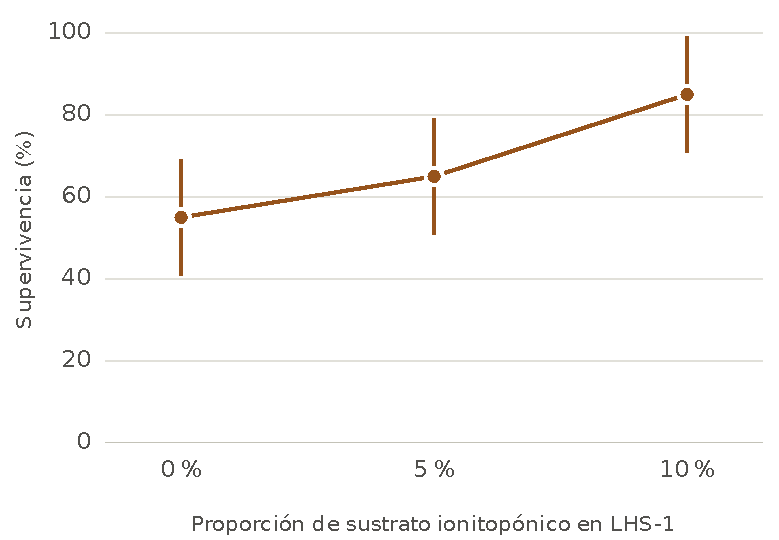
\includegraphics[width=0.72\linewidth]{figA_supervivencia_dosis_es}
\caption{\capFigA}\label{fig:dose}
\end{figure}

\begin{table}[H]
\caption{\capTabB}\label{tab:anova-dose}
\tabla{tabB_anova_dosis_es}
\end{table}

Con respecto al primer componente de la hipótesis (C1), la supervivencia en el simulante enmendado fue, en promedio, 20.0 puntos porcentuales mayor que en LHS-1 sin enmendar (IC 95\,\%: $-15.5$ a 55.5), una diferencia que no alcanzó significancia estadística ($p$ unilateral $= 0.130$; $p$ bilateral $= 0.260$). Con respecto al segundo componente (C2), la supervivencia con 10\,\% de sustrato ionitopónico fue 20.0 puntos porcentuales mayor que con 5\,\% (IC 95\,\%: $-21.0$ a 61.0; $p = 0.328$). Después del ajuste de Holm, los valores $p$ fueron 0.260 y 0.328, respectivamente. Por lo tanto, no se rechazó ninguna de las dos hipótesis nulas (Tabla~\ref{tab:contrasts}, Figura~\ref{fig:forest}).

Al comparar cada proporción con el control sin enmendar, la diferencia fue de 10.0 puntos porcentuales para 5\,\% ($p$ unilateral $= 0.311$) y de 30.0 puntos porcentuales para 10\,\% ($p$ unilateral $= 0.073$; $p$ ajustado por Holm $= 0.146$). Esta última comparación equivale a la tendencia lineal a lo largo de las tres proporciones y corresponde a un aumento estimado de 3.0 puntos porcentuales en la supervivencia por cada 1\,\% adicional de sustrato ionitopónico (IC 95\,\%: $-1.1$ a 7.1).

\begin{table}[H]
\caption{\capTabC}\label{tab:contrasts}
\tabla{tabC_contrastes_es}
\end{table}

\begin{figure}[H]
\centering
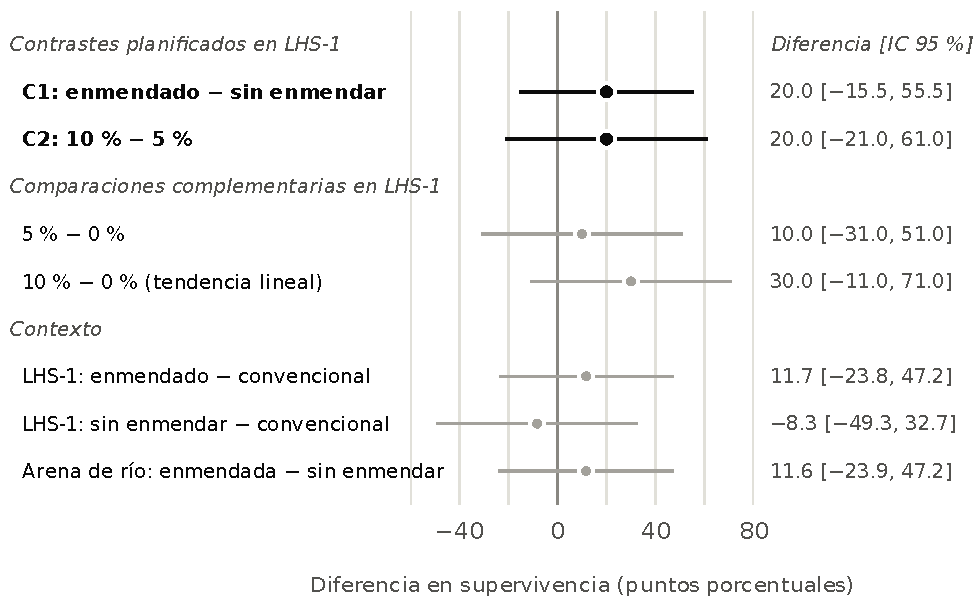
\includegraphics[width=0.95\linewidth]{figB_contrastes_es}
\caption{\capFigB}\label{fig:forest}
\end{figure}

\subsection{Robustez del resultado}

La conclusión no dependió de la forma en que se estimó el error experimental: el valor $p$ unilateral de C1 osciló entre 0.112 y 0.136, y el valor $p$ de C2 osciló entre 0.263 y 0.328 (Tabla~\ref{tab:sensitivity}). A nivel de semilla, la prueba exacta de Fisher condujo a la misma conclusión para C1 (29 de 39 plántulas sobrevivientes en el simulante enmendado frente a 11 de 20 en LHS-1 sin enmendar; $p$ unilateral $= 0.113$) y para C2 (16 de 19 frente a 13 de 20; $p = 0.273$).

La prueba exacta de tendencia a lo largo de las tres proporciones, a nivel de semilla, arrojó un valor $p$ unilateral de 0.038. No obstante, este análisis supone que las semillas de una misma unidad experimental responden de manera independiente, y la variabilidad observada entre unidades fue aproximadamente 1.6 veces mayor que la esperada bajo ese supuesto. Al tomar en cuenta esta sobredispersión, el valor $p$ fue de 0.059, en concordancia con el análisis a nivel de unidad ($p = 0.073$). En consecuencia, la tendencia creciente debe considerarse sugerente y no concluyente.

\begin{table}[H]
\caption{\capTabD}\label{tab:sensitivity}
\tabla{tabD_sensibilidad_es}
\end{table}

\subsection{Contexto de la hipótesis}

La supervivencia en LHS-1 sin enmendar no difirió significativamente de la observada en LHS-1 con solución nutritiva convencional ($-8.3$ puntos porcentuales; $p = 0.683$) ni en arena de río sin enmendar ($+10.0$ puntos porcentuales; $p = 0.623$). De igual manera, el simulante enmendado no difirió significativamente de LHS-1 con solución nutritiva convencional ($+11.7$ puntos porcentuales; IC 95\,\%: $-23.8$ a 47.2; $p = 0.507$). En arena de río, la enmienda se asoció con una diferencia de magnitud similar ($+11.6$ puntos porcentuales; $p = 0.509$), y el efecto de la enmienda no difirió entre sustratos ($p = 0.737$; Tabla~\ref{tab:context}).

\begin{table}[H]
\caption{\capTabE}\label{tab:context}
\tabla{tabE_contexto_es}
\end{table}

\subsection{Supervivencia de plántulas según sustrato y tratamiento}

Considerando el diseño factorial completo, la supervivencia media fue de 67.1\,\% en LHS-1 y de 51.7\,\% en arena de río, una diferencia de 15.4 puntos porcentuales (IC 95\,\%: $-5.1$ a 35.9) que no fue estadísticamente significativa ($F_{1,32} = 2.35$, $p = 0.135$). Tampoco fueron significativos el efecto del tratamiento ($F_{3,32} = 0.83$, $p = 0.489$) ni la interacción entre sustrato y tratamiento ($F_{3,32} = 0.15$, $p = 0.927$) (Tabla~\ref{tab:anova-factorial}, Figura~\ref{fig:factorial}), y ninguna de las comparaciones por pares entre tratamientos alcanzó significancia (prueba de Tukey, $p \ge 0.438$).

\begin{table}[H]
\caption{\capTabF}\label{tab:anova-factorial}
\tabla{tabF_anova_factorial_es}
\end{table}

\begin{figure}[H]
\centering
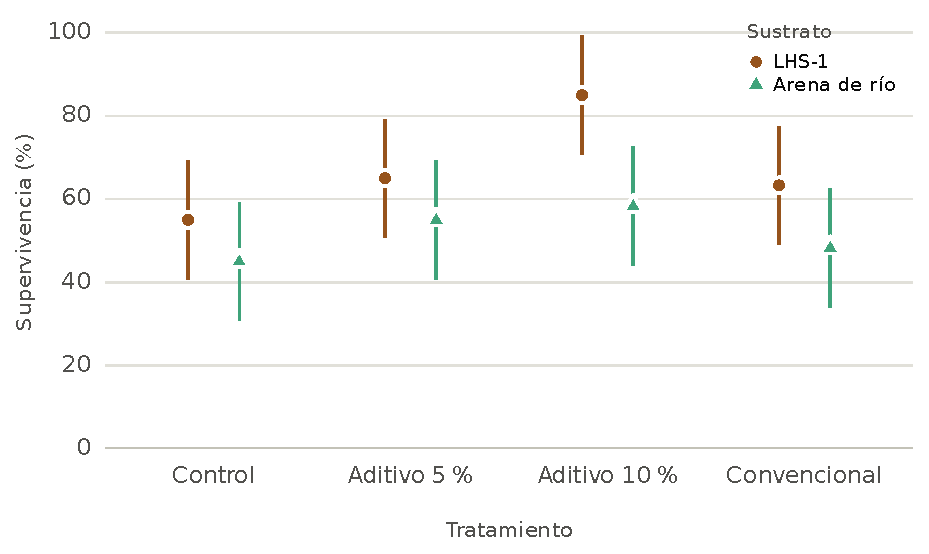
\includegraphics[width=0.85\linewidth]{figC_supervivencia_factorial_es}
\caption{\capFigC}\label{fig:factorial}
\end{figure}

\subsection{Germinación}

La germinación global fue idéntica en ambos sustratos (72 de 80 semillas, 90.0\,\%; diferencia de 0.0 puntos porcentuales, IC 95\,\%: $-9.8$ a 9.8). Los valores más bajos se observaron en LHS-1 con solución nutritiva convencional (13 de 20 semillas, 65.0\,\%) y en arena de río con aditivo al 5\,\% (15 de 20 semillas, 75.0\,\%; Tabla~\ref{tab:germination}, Figura~\ref{fig:germination}).

\begin{table}[H]
\caption{\capTabG}\label{tab:germination}
\tabla{tabG_germinacion_es}
\end{table}

\begin{figure}[H]
\centering
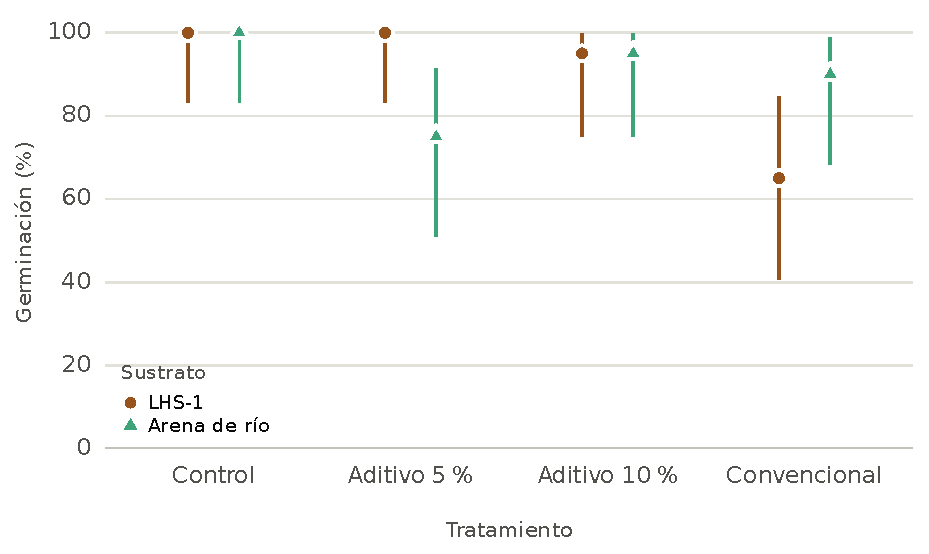
\includegraphics[width=0.85\linewidth]{figD_germinacion_es}
\caption{\capFigD}\label{fig:germination}
\end{figure}

A nivel de semilla, la germinación difirió entre tratamientos (prueba exacta de Fisher, $p = 0.003$), principalmente por la menor germinación observada con la solución nutritiva convencional (31 de 40 semillas frente a 40 de 40 en el control; $p$ ajustado por Holm $= 0.007$). Sin embargo, cuando se tomó la unidad experimental como unidad de análisis, ninguna de las comparaciones alcanzó significancia estadística (Tabla~\ref{tab:germ-contrasts}). Esta diferencia entre los dos niveles de análisis se explica porque las semillas no germinadas en LHS-1 con solución nutritiva convencional se concentraron en tres de las cinco unidades experimentales, una de las cuales no presentó germinación. En concordancia con lo anterior, al tomar en cuenta la sobredispersión en el modelo binomial, la evidencia fue más débil para el efecto del tratamiento ($p$ entre 0.035 y 0.046) y para la interacción entre sustrato y tratamiento ($p$ entre 0.082 y 0.101). Por lo tanto, la menor germinación asociada con la solución nutritiva convencional en LHS-1 debe considerarse una observación preliminar.

\begin{table}[H]
\caption{\capTabH}\label{tab:germ-contrasts}
\tabla{tabH_contrastes_germinacion_es}
\end{table}

\subsection{Integral de luz diaria (DLI)}

No se observó asociación entre el DLI y la supervivencia de plántulas entre las ocho medias de grupo ($r = -0.02$; IC 95\,\%: $-0.71$ a 0.69; $p = 0.964$), ni entre el DLI y la germinación ($r = 0.42$; IC 95\,\%: $-0.40$ a 0.87; $p = 0.295$). Dado que cada ubicación de cultivo albergó tratamientos específicos, el efecto de la luz no puede separarse del efecto de los tratamientos, y estos resultados son únicamente descriptivos.

\section{Interpretación}

Los resultados de la fase piloto son consistentes, en su dirección, con la hipótesis: la supervivencia de plántulas en LHS-1 aumentó progresivamente a medida que aumentó la proporción de sustrato ionitopónico (55.0\,\%, 65.0\,\% y 85.0\,\%). No obstante, con cinco unidades experimentales por grupo, las diferencias observadas no alcanzaron significancia estadística, y los intervalos de confianza fueron amplios: son compatibles tanto con la ausencia de efecto como con una mejora considerable en la supervivencia. En consecuencia, la fase piloto no permite confirmar ni descartar la hipótesis; el resultado debe entenderse como no concluyente y no como evidencia de que la enmienda carece de efecto.

Con los datos de supervivencia disponibles no fue posible verificar la premisa de una baja disponibilidad de nutrientes en LHS-1, dado que la supervivencia en el simulante sin enmendar no fue menor que la observada con la solución nutritiva convencional o en arena de río. Es posible que las variables relacionadas con el desarrollo de las plantas resulten más informativas que la supervivencia para este propósito; este aspecto queda por evaluar. De la misma manera, los datos disponibles no permiten afirmar que la enmienda tenga un desempeño igual al de la solución nutritiva convencional, porque la ausencia de una diferencia significativa no equivale a una demostración de equivalencia.

Con respecto a los sustratos, la germinación fue la misma en LHS-1 y en arena de río, y la supervivencia en LHS-1 no fue menor que en arena de río; el intervalo de confianza de la diferencia ($-5.1$ a 35.9 puntos porcentuales) sugiere que una reducción marcada de la supervivencia atribuible al simulante es poco probable bajo las condiciones evaluadas.

\section{Limitaciones}

Los siguientes aspectos deben considerarse al interpretar estos resultados:

\begin{itemize}[leftmargin=1.4em,itemsep=2pt]
\item \textbf{Tamaño de muestra.} Con cinco unidades experimentales por grupo, la potencia estadística para detectar las diferencias observadas fue baja (0.30 para C1 y 0.16 para C2; Tabla~\ref{tab:power}).
\item \textbf{Número de semillas por unidad.} Con cuatro semillas por unidad, los porcentajes de cada unidad solo pueden tomar unos pocos valores, lo cual limita la precisión de las estimaciones.
\item \textbf{Datos a nivel de resumen.} El análisis se basó en medias y desviaciones estándar; por lo tanto, no fue posible examinar la distribución de los valores por unidad. Además, algunos de los valores de dispersión reportados no pudieron reproducirse exactamente a partir del diseño descrito, por lo que sería recomendable verificarlos con los registros por unidad. Este aspecto no afectó las conclusiones: al utilizar los valores reproducibles más cercanos, el cuadrado medio del error cambió en 2.6\,\% y no se modificó ninguna decisión.
\item \textbf{Ambiente lumínico.} En LHS-1, el grupo con 10\,\% de sustrato ionitopónico se mantuvo en una ubicación de cultivo con un DLI menor (9.52 mol$\cdot$m$^{-2}\cdot$día$^{-1}$) que los grupos control y 5\,\% (10.73 mol$\cdot$m$^{-2}\cdot$día$^{-1}$). En consecuencia, las comparaciones que involucran al grupo de 10\,\% están parcialmente confundidas con la ubicación de cultivo. Únicamente las comparaciones entre 5\,\% y el control, y entre 10\,\% y la solución nutritiva convencional, se realizaron dentro de una misma ubicación.
\item \textbf{Comparaciones exploratorias.} Aparte de los dos contrastes planificados, las demás comparaciones son exploratorias y no se ajustaron conjuntamente por multiplicidad; deben interpretarse como una guía para futuros experimentos.
\end{itemize}

\section{Recomendaciones}

Con base en lo anterior, se sugiere considerar los siguientes puntos para la fase confirmatoria:

\begin{enumerate}[leftmargin=1.6em,itemsep=2pt]
\item \textbf{Aumentar el número de unidades experimentales.} Bajo la variabilidad observada en la fase piloto, se requerirían aproximadamente 24 unidades experimentales por grupo para detectar una diferencia de 20 puntos porcentuales entre el simulante enmendado y sin enmendar con una potencia de 0.80, y aproximadamente 41 unidades por grupo para detectar la misma diferencia entre las dos proporciones (Tabla~\ref{tab:power}, Figura~\ref{fig:power}). Sería preferible definir de antemano la menor diferencia que se considere relevante y calcular el tamaño de muestra a partir de ese valor.
\item \textbf{Aumentar el número de semillas por unidad}, de modo que el porcentaje de cada unidad se estime con mayor precisión.
\item \textbf{Aleatorizar la posición de las unidades} entre las ubicaciones de cultivo, o disponer todos los tratamientos dentro de cada ubicación a manera de bloques y, de ser posible, registrar el DLI de cada unidad. Esto permitiría separar el efecto de la luz del efecto de los tratamientos.
\item \textbf{Registrar y analizar los conteos de cada unidad} (semillas sembradas, germinadas y sobrevivientes). Con estos datos, la germinación y la supervivencia podrían analizarse con un modelo mixto binomial que incluya la unidad experimental como efecto aleatorio, que es el enfoque más apropiado para este tipo de respuesta.
\item \textbf{Incluir variables de desarrollo de las plantas}, de modo que pueda evaluarse el componente de la hipótesis relacionado con el desarrollo.
\item \textbf{Definir el análisis antes del experimento}: la variable de respuesta principal, los contrastes planificados y el nivel de significancia.
\item \textbf{Si el objetivo es mostrar que la enmienda tiene un desempeño comparable al de la solución nutritiva convencional}, definir de antemano el margen de diferencia que se considere aceptable y aplicar una prueba de equivalencia o de no inferioridad.
\item \textbf{Considerar proporciones adicionales de sustrato ionitopónico}, lo cual permitiría describir con mayor detalle la forma de la respuesta.
\end{enumerate}

\begin{table}[H]
\caption{\capTabI}\label{tab:power}
\tabla{tabI_potencia_es}
\end{table}

\begin{figure}[H]
\centering
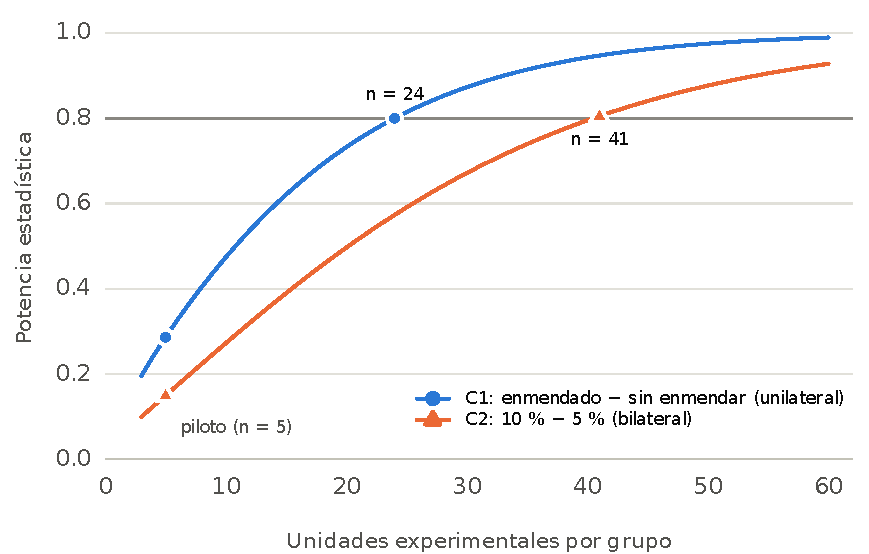
\includegraphics[width=0.8\linewidth]{figE_potencia_es}
\caption{\capFigE}\label{fig:power}
\end{figure}

\begin{thebibliography}{9}
\bibitem[Clopper y Pearson(1934)]{clopper} Clopper, C. J., \& Pearson, E. S. (1934). The use of confidence or fiducial limits illustrated in the case of the binomial. \textit{Biometrika}, 26(4), 404--413.
\bibitem[Holm(1979)]{holm} Holm, S. (1979). A simple sequentially rejective multiple test procedure. \textit{Scandinavian Journal of Statistics}, 6(2), 65--70.
\bibitem[Hurlbert(1984)]{hurlbert} Hurlbert, S. H. (1984). Pseudoreplication and the design of ecological field experiments. \textit{Ecological Monographs}, 54(2), 187--211.
\bibitem[Newcombe(1998)]{newcombe} Newcombe, R. G. (1998). Interval estimation for the difference between independent proportions: comparison of eleven methods. \textit{Statistics in Medicine}, 17(8), 873--890.
\bibitem[R Core Team(2024)]{rcore} R Core Team (2024). \textit{R: A language and environment for statistical computing}. R Foundation for Statistical Computing, Viena, Austria.
\bibitem[Satterthwaite(1946)]{satterthwaite} Satterthwaite, F. E. (1946). An approximate distribution of estimates of variance components. \textit{Biometrics Bulletin}, 2(6), 110--114.
\bibitem[Welch(1947)]{welch} Welch, B. L. (1947). The generalization of ``Student's'' problem when several different population variances are involved. \textit{Biometrika}, 34(1--2), 28--35.
\end{thebibliography}

\end{document}
